\documentclass[../../DS]{subfiles}

\begin{document}
\begin{sloppy}
    
\section{图}

    \textbf{基本定义} \\
    数学定义: 图$G$由顶点$V$和边$E$组成, 记为$G=(V, E)$. $V(G)$表示$G$中顶点的非空子集, $E(G)$表示$G$的边. $V = \{v_1, v_2, \dots\}$, $E = \{(u, v) | u \in V, v \in V\}$. \textbf{图的顶点数(图的阶数)}: $|V|$, \textbf{图的边数}: $|E|$ \\
    图不可以是空图, 图\textbf{至少有一个结点}. 顶点集$V$一定非空, 边集\textbf{可以为空} \\
    \textbf{弧}: 有向边, 顶点的有序对, 记为$<v, w>$, $v \to w$, \textbf{弧尾}: $v$, \textbf{弧头}: $w$. 称: $<v, w>$为v到w的弧, 或$v$ 邻接\textbf{到} $w$ \\
    \textbf{边}: 无向边. 记为$(v, w)$或者$(w, v)$. $v, w$互为 \textbf{邻接点}, 称: 边$(v, w)$依附于w和v, 或者边$(v, w)$与$v, w$相关联 \\
    \textbf{简单图(存在有向无向之分)}: 1. 不存在重复边; 2. 不允许顶点到自身的边 \\
    \textbf{复杂图}: 存在重复边或者存在顶点到自身的边 \\
    \textbf{顶点的度}: \\
    \textbf{无向图}: 顶点$v$的度是依附于$v$的边的数量, 记为$TD(v)$. \textbf{无向图}全部顶点的度之和为边数的2倍(一条边连接两个顶点), 即$\sum\limits_{i=1}^{n}TD(v_i) = 2 |E|$ \\
    \textbf{有向图}: 区分\textbf{入度}, \textbf{出度}, \textbf{度}. \\
    \textbf{入度}: 以$v$为终点的边的数量, 记作$ID(v)$. \textbf{出度}: 以$v$为起点的边的数量, 记作$OD(v)$. \\
    \textbf{度}: 入度与出度之和, 记作$TD(v) = ID(v) + OD(v)$. 有向图中: $\sum\limits_{i=1}^{n}ID(v_i) = \sum\limits_{i=1}^{n}OD(v_i) = |E|$ \\
    \textbf{路径}: 顶点$v_p$到$v_q$之间的序列$v_p, v_1, v_2, \dots, v_q$ \\
    \textbf{路径长度}: 路径上边的数目 \\
    \textbf{回路(环)}: 首末顶点相同的路径. 若一个图有$n$个顶点, 有多于$n-1$条边, 则该图\textbf{一定有环} \\
    \textbf{简单路径}: 顶点不重复出现的路径 \\
    \textbf{简单回路}: 除了首末顶点之外, 其他顶点不重复出现的回路 \\
    \textbf{距离(区分有向无向)}: 从$u$\textbf{到}$v$的\textbf{最短}路径长度. 若$u, v$之间不存在路径, 则距离为无穷$\infty$ \\
    \textbf{子图}: 若$G = (V, E), G' = (V', E')$, $V'$是$V$的子集, $E'$是$E$的子集, 则$G'$是$G$的子图. 若要构成子图, 则$E'$涉及的顶点必须全在$V'$中, 否则不构成图, 因此, 不是VE的任何子集都能构成G的子图 \\
    \textbf{生成图}: $G'$是$G$的子图, 且$V(G') = V(G)$, 即子图包含原图的全部顶点 \\
    \textbf{连通}: \textbf{无向图中}, 顶点v和w之间存在\textbf{路径}. \\
    \textbf{连通图}: 无向图中任意两个顶点都是连通的; \textbf{非连通图}: 不是连通图的无向图. \textbf{极大连通子图(连通分量)}: 1. 连通图; 2. 包含尽可能多的顶点和边(\textbf{不能被任何另外一个连通子图所包含}) \\
    对于有$n$个顶点的无向图, 若为\textbf{连通图}, \textbf{最少有} n-1条边(一个顶点连接所有); 若保证为\textbf{非连通图}, \textbf{最多有} $\binom{n-1}{2}$条边(n-1个顶点两两相连, 孤立一个顶点) \\
    \textbf{强连通}: \textbf{有向图}中, 对于顶点v, w, 从v到w和从w到v的路径都存在(不一定有$<v, w>$或$<w, v>$), 则称这两个顶点强连通 \\
    \textbf{强连通图}: 有向图中, 任意两个顶点都是强连通的 \\
    \textbf{强连通分量}: 1. 强连通图; 2. 包含尽可能多的顶点和边. 若一个图是强连通图, \textbf{最少有}n条边(构成环) \\
    \textbf{生成树}: \textbf{连通图}中包含图中全部顶点的一个\textbf{极小连通子图}. 1. 包含全部顶点; 2. 边尽可能少. n个顶点的图, 其生成树只能有n-1条边. 生成树可能有多个 \\
    \textbf{生成森林}: \textbf{非连通图}中, 连通分量的生成树构成非连通图的生成森林 \\
    \textbf{边的权值}: 每条边都可以标注的有意义的数值 \\
    \textbf{网(带权图)}: 边有权值的图 \\
    \textbf{带权路径长度}: 路径上所有边的权值之和
    
    \newpage
    \noindent
    \textbf{完全图(简单完全图)}: 对于n个顶点的\textbf{无向图}, 有$\binom{n}{2} =  \frac{n(n-1)}{2}$条边的图(任意两个顶点之间有边); 对于n个顶点的\textbf{有向图}, 有$2 \binom{n}{2} = n(n-1)$条边的图(任意两个顶点之间有方向相反的两条边). n个顶点, 无向图, 边的条数$\in[0, \binom{n}{2}]$; 有向图, 边的条数$[0, n(n-1)]$ \\
    \textbf{稠密图}: 边很多的图; \textbf{稀疏图}: 边很少的图. 一般, 满足$|E| < |V| \log_2 |V|$可视为稀疏图(没有绝对的判断标准) \\
    \textbf{有向树}: 一个顶点的入度为0, 其余顶点的入度均为1的有向图(不是强连通图) \\
    \textbf{树}: 1. 无向图; 2. 不存在回路; 3. 连通; 

    \begin{figure}[htbp]
        \centering
        \includegraphics[width=0.5\columnwidth]{./graphconnect.png}
    \end{figure}

    \textbf{找强连通分量} \\
    1. 分离出孤立顶点 \\
    2. 分离出没有出度的顶点和与其相连的边 \\
    3. 分离出没有入度的顶点和与其相连的边

    \begin{figure}[htbp]
        \centering
        \begin{subfigure}{0.45\textwidth}
            \begin{tikzpicture}[node distance=1.5cm, , >=Stealth]
                \tikzstyle{vertex}=[circle, draw, minimum size=0.5cm]
            
                \node[vertex] (A) {A};
                \node[vertex, below right of=A] (D) {D};
                \node[vertex, above right of=D] (C) {C};
                \node[vertex, below left of=D] (B) {B};
                \node[vertex, below right of=D] (E) {E};
                \node[vertex, below left of=A] (F) {F};
                \node[vertex, below right of=C] (G) {G};
                
                \draw[->] (A) to[bend left=20] (C);
                \draw[->] (C) to[bend left=20] (A);
                \draw[->] (B) -- (A);
                \draw[->] (D) -- (A);
                \draw[->] (C) -- (D);
                \draw[->] (D) -- (E);
                \draw[->] (E) -- (C);
                \draw[->] (B) -- (D);
                \draw[->] (B) -- (E);
                \draw[->] (C) -- (G);
                \draw[->] (E) -- (G);
            \end{tikzpicture}
            \caption{有向图}
        \end{subfigure}
        \begin{subfigure}{0.45\textwidth}
            \begin{tikzpicture}[node distance=1.5cm, , >=Stealth]
                \tikzstyle{vertex}=[circle, draw, minimum size=0.5cm]
                
                \node[vertex] (A) {A};
                \node[vertex, below right of=A] (D) {D};
                \node[vertex, above right of=D] (C) {C};
                \node[vertex, below right of=D] (E) {E};
                \node[vertex, below left of=A] (F) {F};
                \node[vertex, below right of=C] (G) {G};
                \node[vertex, right of=G] (B) {B};

                \draw[->] (A) to[bend left=20] (C);
                \draw[->] (C) to[bend left=20] (A);
                \draw[->] (D) -- (A);
                \draw[->] (C) -- (D);
                \draw[->] (D) -- (E);
                \draw[->] (E) -- (C);
            \end{tikzpicture}
            \caption{4个强连通分量}
        \end{subfigure}
    \end{figure}

\subsection{图的存储}

\subsubsection{邻接矩阵法}

    顺序存储. 用一个一维数组存储图中顶点的信息, 用一个二维数组存储图中边的信息, 其中, 二维数组称为\textbf{邻接矩阵}. 在简单应用中, 可以忽略一维数组, 不存储顶点信息. 邻接矩阵的空间复杂度为$O(|V|^2)$. \textbf{稠密图}适合使用邻接矩阵 
    图中, 顶点自身与自身不认为有边连接. 记有n个顶点的图之顶点为$v_1, v_2, \dots, v_n$

    \textbf{非带权图}
    
    % new two columns
    \vspace{-2\baselineskip}
    \begin{center}
    \begin{minipage}[t]{0.48\textwidth}
    \vspace{0pt}
    \begin{center}
        $
        A[i][j] = \begin{cases}
            1, <v_i, v_j>\mbox{或}(v_i, v_j)\mbox{是图中的边} \\
            0, <v_i, v_j>\mbox{或}(v_i, v_j)\mbox{不是图中的边} \\
        \end{cases}
        $
    \end{center}
    \end{minipage}
    \begin{minipage}[t]{0.48\textwidth}
    \vspace{0pt}
        注意i, j的先后关系在有向图中不可以对换. \textbf{有向图}中 \verb|A[i][j]|是边 \verb|i->j|. \textbf{无向图}中, 邻接矩阵是一个\textbf{唯一的}对称矩阵(上下三角压缩存储)
    \end{minipage}
    \end{center}

    \vspace{-1\baselineskip}
    \textbf{带权图}

    % new two columns
    \vspace{-2\baselineskip}
    \begin{center}
    \begin{minipage}[t]{0.53\textwidth}
    \vspace{0pt}
    \begin{center}
        $
        A[i][j] = \begin{cases}
            w_{ij}, <v_i, v_j>\mbox{或}(v_i, v_j)\mbox{是图中的边} \\
            0 \mbox{或} \infty, <v_i, v_j>\mbox{或}(v_i, v_j)\mbox{不是图中的边} \\
        \end{cases}
        $
    \end{center}
    \end{minipage}
    \begin{minipage}[t]{0.45\textwidth}
    \vspace{0pt}
        1. $\infty$可以定义为 \verb|MAXINT|; 2. 部分情况下, 自身与自身(对角线): 0, 无边: $\infty$
    \end{minipage}
    \end{center}

    \newpage
    \textbf{数据结构}
    \begin{lstlisting}[style = Cpp]
    struct MGgraph {
        VertexType vex[MaxVertexNum];                 // 顶点表
        EdgeType edge[MaxVertexNum][MaxVertexNum];    // 邻接矩阵(边表)
        int vexnum, arcnum;                           // 图当前的顶点数和边数
    };
    \end{lstlisting}

    \vspace{-0.5\baselineskip}
    \textbf{邻接矩阵有关计算} \\
    1. \textbf{无向图}: 顶点的度$TD(v_i)$为矩阵中第$i$行或者第$i$列非零($\infty$)元素的个数 \\
    2. \textbf{有向图}: 顶点$v_i$的\textbf{入度}$ID(v_i)$为第$i$\textbf{列}非零($\infty$)元素的个数; \textbf{出度}$OD(v_i)$为第$i$\textbf{行}非零($\infty$)元素的个数 \\
    3. 设图$G$的领接矩阵为$A$, 则$A^n[i][j]$表示有顶点$i$到顶点$j$, 长度为$n$的路径的条数 \\
    EX. $A^2[1][4] = a_{11} a_{14} + a_{12} a_{24} + a_{13} a_{34} + a_{14} a_{44}$, 一个因子为1, 则 \verb|i->k->j|路径存在 \\
    邻接矩阵容易确定任意两个顶点之间是否有边连接, 但是确定图中有几条边, 需要按行和按列进行遍历每一个元素. $T(n) = O(|V|^2)$. \\
    邻接矩阵计算顶点的度$T(n) = O(|V|)$

    \begin{figure}[htbp]
        \centering
        \includegraphics[width=0.5\columnwidth]{./matrix.png}
    \end{figure}
    
    

\subsubsection{邻接表法}

    \vspace{-1\baselineskip}
    顺序存储+链式存储. 当存储稀疏图时, 可以减少大量空间浪费. 对每个顶点建立一个单链表, 称为\textbf{边表}(有向图中称为\textbf{出边表}), 边表表示依附于顶点$v_i$的边或者以$v_i$为尾的弧(有向图). 顶点的数据信息和边表的头指针使用\textbf{顺序存储}. \\
    若为\textbf{无向图}, $S(n) = O(|V| + 2|E|)$(每条边出现两次); \textbf{有向图}: $S(n) = O(|V| + |E|)$

    \begin{lstlisting}[style = Cpp]
        // 边表结点
        struct ArcNode
        {
            int adjvex;              // 该边指向的顶点
            struct ArcNode *nextarc; // 下一条边
        };
        // 顶点表结点
        struct VNode
        {
            VertexType data;   // 顶点信息
            ArcNode *firstarc; // 指向第一条边或者弧的指针
        };
        // 邻接表
        struct ALGraph
        {
            VNode vertices[MaxVertexNum];  // 边表
            int vexnum, arcnum;            // 顶点数和边数
        };
    \end{lstlisting}

    \newpage
    \textbf{计算度} \\
    1. \textbf{无向图}: 遍历顶点$v_i$的边表 \\
    2. \textbf{有向图}: \textbf{出度}: 遍历顶点$v_i$的出边表; \textbf{入度}: 遍历全部顶点的出边表

    \begin{note}
        1. 有向图找出边方便, 找入边麻烦. 无向图找边方便. 若要确定两个顶点中是否右边, 需要在一个顶点的边表中找另一个顶点, 效率低 \\
        2. 图的邻接表\textbf{不唯一}, 各边结点的链接次序任意    
    \end{note}
    

\subsubsection{十字链表}

    十字链表用于存储\textbf{有向图}, \textbf{顺序+链式存储}. 每条弧用弧结点存, 每个顶点用顶点节点存, 顶点结点为顺序存储. 十字链表\textbf{不唯一}. $S(n) = O(|V| + |E|)$. 从任意顶点出发, 能够快速遍历出边和全部入边, 求度方便.

    \vspace{-1.5\baselineskip}
    % new two columns
    \begin{center}
    \begin{minipage}[t]{0.48\textwidth}
    \vspace{0pt}
        \begin{center}
        弧结点

        \begin{tabular}{|c|c|c|c|c|}
        \hline
        tailvex & headvex & hlink & tlink & (info) \\
        \hline 
        \end{tabular}
        \end{center}

        \noindent
        tailvex: 弧尾顶点编号 \\
        headvex: 弧头顶点编号 \\
        hlink: 相同弧头的下一条弧(顶点的下一条入边) \\
        tlink: 相同弧尾的下一条弧(顶点的下一条出边)
        
    
    \end{minipage}
    \begin{minipage}[t]{0.48\textwidth}
    \vspace{0pt}
        \begin{center}
        顶点结点 

        \begin{tabular}{|c|c|c|}
        \hline
        data & firstin & firstout \\
        \hline
        \end{tabular}
        \end{center}
        
        \noindent
        firstin: 顶点的第一条入边(以该顶点为弧头的弧) \\
        firstout: 顶点的第一条出边(以该顶点为弧尾的弧)

    
    \end{minipage}
    \end{center}

    \begin{figure}[htbp]
        \centering
        \includegraphics[width=0.7\columnwidth]{./crosslink.png}
    \end{figure}

    画图或编写算法时, 可以先把出边全部处理完, 再以此链接每个结点的入边表.

\newpage
\subsubsection{邻接多重表}

    邻接多重表用于存储\textbf{无向图}, \textbf{顺序+链式存储}. 边存储于边结点中, 顶点存储于顶点结点中(顺序). 容易求得顶点和边的各种信息, 但是求两个顶点之间是否存在边和删除边时, 需要分别从两个结点开始遍历边表, 效率低. 

    由于每条边依附于两个顶点, 因此, 每个边结点同时链接在两个顶点的链表中. 无向图的邻接多重表和邻接表的唯一区别: \textbf{邻接表}中同一条边有分属于两个链表中的两个结点, \textbf{邻接多重表中}只有一个结点

    \vspace{-1.5\baselineskip}
    % new two columns
    \begin{center}
    \begin{minipage}[t]{0.48\textwidth}
    \vspace{0pt}
        \begin{center}
        边结点

        \begin{tabular}{|c|c|c|c|c|}
        \hline
        ivex & ilink & jvex & jlink & (info) \\
        \hline 
        \end{tabular}
        \end{center}

        \noindent
        ivex, jvex: 顶点i, j的编号 \\
        ilink, jlink: 依附于顶点i, j的下一条边
        
    
    \end{minipage}
    \begin{minipage}[t]{0.48\textwidth}
    \vspace{0pt}
        \begin{center}
        顶点结点 

        \begin{tabular}{|c|c|}
        \hline
        data & firstedge \\
        \hline
        \end{tabular}
        \end{center}
        
        \noindent
        firstedge: 依附于该顶点的第一条边

    
    \end{minipage}
    \end{center}

    \begin{figure}[htbp]
        \centering
        \includegraphics[width=0.7\columnwidth]{nondirectcrosslink.png}
    \end{figure}
    
    画图或编写算法时, 可以每个顶点依次新增或链接完全衣服于该结点的边. 注意结点每个成员的意义, 链接边的时候注意链接到成员ilink还是jlink.

    \begin{center}
        \textbf{图存储方式总结}

        \begin{tabular}{c|c|c|c|c}
        \toprule
        {} & 邻接矩阵 & 邻接表 & 十字链表 & 邻接多重表 \\
        \midrule
        空间复杂度 & $O(|V|^2)$ & \makecell{无向图: $O(|V| + 2|E|)$ \\ 有向图: $O(|V| + |E|)$} & $O(|V| + |E|)$ & $O(|V| + |E|)$ \\
        \midrule
        找相邻边 & 遍历行/列, $T(n) = O(|V|)$ & 有向图\makecell{找出边遍历结点出边表 \\ 找入度遍历整个邻接表} & 方便 & 方便 \\
        \midrule
        删除边或顶点 & \makecell{删除边方便\\ 删除顶点需要移动大量元素} & \makecell{无向图中删除边或者顶点都要 \\ 遍历两个顶点的边表, 不方便} & 方便 & 方便 \\
        \midrule
        适用 & 稠密图 & 都行 & 有向图 & 无向图 \\
        \midrule
        表示方式 & 唯一 & 不唯一 & 不唯一 & 不唯一 \\
        \bottomrule        
        \end{tabular}
    \end{center}
    
\newpage
\subsection{图的基本操作}

    \noindent
    Adjacent (G, x, y):判断图 G 是否存在边<x, y>或 (x, y)。\\
    \indent 邻接矩阵: $O(1)$; 邻接表: 最好$O(1)$, 最坏$O(|V|-1)=O(|V|)$ \\
    Neighbors (G, x): 列出图 G 中与结点 x 邻接的边。\\
    \indent 邻接矩阵: $O(|V|)$; 邻接表: $O(1) \sim O(|V|)$. 其中有向图, 出边$O(1) \sim O(|V|)$, 入边: $O(|E|)$ \\
    InsertVertex (G,x): 在图 G 中插入顶点 x 。\\
    \indent $T(n) = O(1)$ \\
    DeleteVertex (G, x): 从图 G 中删除顶点 x 。\\
    \indent 邻接矩阵: $O(|V|)$(顶点x的行列全部置零, 再标记顶点已删除); 邻接表: $O(1) \sim O(|E|)$. \\
    AddEdge (G, x, y):若无向边 (x, y)或有向边<x, y>不存在,则向图 G 中添加该边。\\
    \indent $T(n) = O(1)$ \\
    RemoveEdge (G, x, y):若无向边 (x, y)或有向边<x, y>存在,则从图 G 中删除该边。\\
    \indent 邻接矩阵: $O(|1|)$; 邻接表: $O(1) \sim O(|V|)$. \\
    FirstNeighbor (G, x): 求图 G 中顶点 x 的第一个邻接点,若有则返回顶点号。若x没有邻接点或图中不存在 x, 则返回-1 。\\
    \indent 邻接矩阵: $O(1) \sim O(|V|)$; 邻接表: 无向图: $O(1)$, 有向图: 出边$O(1)$, 入边$O(1) \sim O(|E|)$. \\
    NextNeighbor(G,x, y):假设图 G 中顶点y是顶点 x 的一个邻接点,返回除y外顶点 x 的下一个邻接点的顶点号,若y是 x 的最后一个邻接点,则返回- 1 。\\
    \indent 邻接矩阵: $O(|1|) \sim O(|V|)$; 邻接表: $O(1)$. \\
    Get\_edge\_value (G, x, y): 获取图 G 中边 (x, y)或<x, y>对应的权值。\\
    \indent 时间在于找边, 复杂度同Adjacent \\ 
    Set\_edge\_value (G,x, y ,v): 设置图 G 中边 (x, y)或<x, y>对应的权值为 v 。\\
    \indent 时间在于找边, 复杂度同Adjacent

\subsection{图的遍历}

    图在遍历过程中, 需要一个辅助数组 \verb|bool visited[numVertives]|来记录顶点是否已经访问过. 

\subsubsection{广度优先搜索 BFS}

    \vspace{-1\baselineskip}
    类似于树的层序遍历. 对于每个结点, 先访问, 标记为已访问后, 入队; 结点出队时, 访问其全部邻接的未访问结点. BFS需要借助辅助队列实现.

    \begin{lstlisting}[style = Cpp]
        bool visited[MaxVertexNum];
        SqQueue Q;
        void BFSTraverse(Graph G)
{
            int i;
            for (i=0; i<G.vexnum; i++) // 初始化辅助数组
                visited[i] = false;
            InitQueue(Q);
            for (i=0; i<G.vexnum; i++) // 对每个连通分量都调用一次
                if (!visited[i])
                    BFS(G, i);
        }
    \end{lstlisting}


    \newpage

    % new two columns
    \begin{center}
    \begin{minipage}[t]{0.5\textwidth}
    \vspace{0pt}
        \textbf{邻接表实现}
        
        \begin{lstlisting}[style = Cpp]
            void BFS (ALGraph G, int i)
            {
                int v, w; // 工作结点
                ArcNode* p; // 用于访问邻接点
                // 访问初始结点
                visit(G, i);
                visited[i] = true;
                EnQueue(Q, i);
                while (!QueueEmpty(Q)) { 
                    DeQueue(Q, v); // 队首结点
                    for (p=G.vertices[v].firstarc; p; p=p->nextarc) { // 遍历全部邻接点
                        w = p->adjvex;
                        if (!visited[w]) { // 未被访问
                            visit(G, w);
                            visited[w] = true;
                            EnQueue(Q, w);
                        }
                    }
                }    
            }
        \end{lstlisting}
    \end{minipage}
    \begin{minipage}[t]{0.45\textwidth}
    \vspace{0pt}
        \textbf{邻接矩阵实现}

        \begin{lstlisting}[style = Cpp]
            void BFS(MGgraph G, int i)
            {
                int v, w; // 工作节点
                // 访问初始结点
                visit(G, i);
                visited[i] = true;
                EnQueue(Q, i);
                while (!QueueEmpty(Q)) {
                    DeQueue(Q, v); // 队首结点
                    for (w=0; w<G.vexnum; w++) { // 遍历全部邻接点
                        if (!visited[w] && G.edge[v][w] == 1) { // 未被访问且<v, w>or(v, w)有边
                            visit(G, w);
                            visited[w] = true;
                            EnQueue(Q, w);
                        }
                    }
                }
            }
        \end{lstlisting}
    \end{minipage}
    \end{center}
    
    \textbf{单源最短路径}

    对于\textbf{非带权图和权重均相等的图}, 可以使用BFS搜索单源最短路径. 对于带权图, 只能使用Floyd和Dijkstra.

    \begin{lstlisting}[style = Cpp]
        int d[MaxVertexNum]; // 记录源点到该点的最短路径长度
        int path[MaxVertexNum]; // 记录该点在最短路径上的直接前驱
        void BFS_Min_Path(Graph G, int u){
            int w; // 工作结点
            for (int i=0; i<G.vexnum; i++) // 初始化路径长度为无穷
                d[i] = INT32_MAX;
            visited[u] = true;
            d[u] = 0;
            EnQueue(Q, u);
            while (!QueueEmpty(Q)) {
                DeQueue(Q, u);
                for (w=FirstNeighbor(G, u); w>0; w=NextNeighbor(G, u, w)) {
                    if (!visited[w]) { // 未被访问
                        visited[w] = true;
                        EnQueue(Q, w);
                        d[w] = d[u] + 1; // 在上一层长度基础上+1
                        path[w] = u; // 记录w的前驱
                    }
                }
            }
        
        }
    \end{lstlisting}

    \newpage
    \textbf{性能分析}

    \noindent
    \textbf{空间复杂度}: 需要借助辅助队列, 最坏情况下$|V| - 1$个结点在第二次入队时入队. $S(n) = O(|V|)$ \\
    \textbf{时间复杂度}: \\
    邻接矩阵: $T(n) = O(|V| + |V|^2) = O(|V|^2)$ (遍历顶点 + 遍历边表); \\
    邻接表: 有向: $T(n) = O(|V| + |E|)$, 无向: $T(n) = O(|V| + 2|E|)$

    \textbf{广度优先生成树}

    将遍历过程分层, 可以得到遍历树, 称为广度优先生成树. 该遍历树是指定顶点为根的树中, 高度最小的生成树. 同时, 层次也反映了从源点出发到各个顶点的最短距离. 对于同一个图, 邻接矩阵的表示是唯一的, 广度优先生成树也是唯一的; 邻接表不唯一, 其广度优先生成树亦不唯一. 对于非(强)连通图, 遍历时会产生广度优先生成森林.

\subsubsection{深度优先搜索DFS}

    DFS是一个递归算法, 需要使用递归工作栈.

    \begin{lstlisting}[style = Cpp]
        void DFSTraverse (Graph G)
        {
            int i;
            for (i=0; i<G.vexnum; i++) // 初始化辅助数组
                visited[i] = false;
            for (i=0; i<G.vexnum; i++) // 对每个连通分量都调用一次
                if (!visited[i])
                    DFS(G, i);
        }
    \end{lstlisting}

    % new two columns
    \begin{center}
    \begin{minipage}[t]{0.5\textwidth}
    \vspace{0pt}
        \textbf{邻接表实现}

        \begin{lstlisting}[style = Cpp]
            void DFS(ALGraph G, int i)
            {
                ArcNode* p; // 工作结点
                int j;
                visit(G, i);
                visited[i] = true;
                for (p=G.vertices[i].firstarc; p; p=p->nextarc) { // 访问全部邻接点
                    j = p->adjvex;
                    if (!visited[j]) // 未被访问
                        DFS(G, j);
                }
            }
        \end{lstlisting}
    \end{minipage}
    \begin{minipage}[t]{0.45\textwidth}
    \vspace{0pt}
        \textbf{邻接矩阵实现}
        
        \begin{lstlisting}[style = Cpp]
            void DFS (MGgraph G, int i)
            {
                int j; // 工作顶点
                visit(G, i);
                visited[i] = true;
                for(j=0; j<G.vexnum; j++) { // 遍历各邻接点
                    if (!visited[j] && G.edge[i][j] == 1) // 未被访问且有边
                        DFS(G, j);
                }
            }
        \end{lstlisting}
    \end{minipage}
    \end{center}
    
    \newpage
    \textbf{性能分析}
    
    \noindent
    \textbf{空间复杂度}: 需要使用递归工作栈, $S(n) = O(|V|)$ \\
    \textbf{时间复杂度}: \\
    邻接矩阵: $T(n) = O(|V|^2)$ \\
    邻接表: 有向图: $T(n) = O(|V| + |E|)$; 无向图: $T(n) = O(|V| + 2|E|)$

    \textbf{深度优先生成树}

    (强)连通图会产生深度优先生成树; (强)非连通图会生成深度优先生成森林. 

    \subsubsection{图的遍历与连通性}
    
    \textbf{Traverse过程中, BFS/DFS的调用次数 = 图的连通分量个数}

    对于\textbf{无向图}: 只需要一次遍历就能访问全部, 则是连通图; 否则为非连通图, 并且每次遍历能够访问该连通分量的全部顶点

    \textbf{对于有向图}: 由于分为强连通分量和非强连通分量, 在非强连通分量中, 一次遍历不一定能访问该子图的全部顶点.

    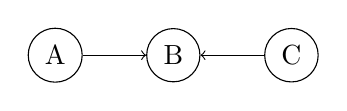
\begin{tikzpicture}[node distance=1.5cm]
        \tikzstyle{vertex}=[circle, draw, minimum size=0.6cm]
    
        \node[vertex] (A) {A};
        \node[vertex, right of=A] (B) {B};
        \node[vertex, right of=B] (C) {C};
        
        \draw[->] (A) -- (B);
        \draw[->] (C) -- (B);
    \end{tikzpicture}

\end{sloppy}
\end{document}